\documentclass[12pt,oneside,a4paper]{report}
\usepackage[OT4]{polski}
\usepackage[cp1250]{inputenc}
\usepackage{geometry}
\usepackage{latexsym}
\usepackage{graphicx}
\usepackage{float}
\usepackage{indentfirst}
\usepackage{hyperref} % paczka do hiper��czy
\usepackage{geometry}
%\usepackage{showframe}
\usepackage{sidecap} % paczka do wstawiania opis�w zdj��
\usepackage{wrapfig} % paczka do op�ywania zdj��
\usepackage{pdfpages}
\usepackage{listings}
\usepackage{mathrsfs}
%\usepackage{verbatim}
\lstset{language=Matlab}



\geometry{marginparwidth=0mm,
left=25mm,
right=25mm,
top=25mm,
bottom=30mm,
footskip=15mm}

%Create by Marek Ogonowski

\makeatletter %w��cza u�ycie "zmiennych" typu \author,\title

%definicja wlasnego przesuniecia PW itd.
\newcommand{\odstep}{\hspace{1,5cm}}

%zdefiniowanie komendy rysujacej linie
\newcommand{\linia}{\rule{\linewidth}{0.4mm}}

%definicja zmienej \place
\newcommand{\place}[1]{\gdef\@place{#1}}%
\newcommand{\@place}{\@latex@warning@no@line{No \noexpand\place given}}

%definicja zmiennej promotor
\newcommand{\promotor}[1]{\gdef\@promotor{#1}}%
\newcommand{\@promotor}{\@latex@warning@no@line{No \noexpand\promotor given}}

%definicja zmiennej nr albumu
\newcommand{\album}[1]{\gdef\@album{#1}}%
\newcommand{\@album}{\@latex@warning@no@line{No \noexpand\album given}}

%definicja zmiennej kierunek studi�w
\newcommand{\kierunek}[1]{\gdef\@kierunek{#1}}%
\newcommand{\@kierunek}{\@latex@warning@no@line{No \noexpand\kierunek given}}

%definicja zmiennej nr albumu
\newcommand{\specjalnosc}[1]{\gdef\@specjalnosc{#1}}%
\newcommand{\@specjalnowsc}{\@latex@warning@no@line{No \noexpand\specjalnosc given}}

%definicja zmienej przedmiot
\newcommand{\przedmiot}[1]{\gdef\@przedmiot{#1}}%
\newcommand{\@przedmiot}{\@latex@warning@no@line{No \noexpand\przedmiot given}}

%zmiana definicji strony tytu�owej
\renewcommand{\maketitle}{\begin{titlepage}

	\begin{figure}
	\vspace*{-1cm}
		\begin{center}

			
\includegraphics[scale=0.08]{PW}
			\qquad
			\hspace*{10cm}
			
\includegraphics[scale=0.08]{OKNO}
		\end{center}	
	\end{figure}
	
	\vspace*{-1,2cm}	
	\noindent\linia

	\vspace*{-3,7cm}
	\begin{center}
		\odstep
    	\textbf{\Large {POLITECHNIKA WARSZAWSKA}}
    	\\[10pt]  \odstep
    	\textbf{O�RODEK KSZTA�CENIA NA ODLEG�O��} 
    	\\ \odstep
    	\\[7pt] \odstep 
    	\normalsize {\@przedmiot}
    \end{center} 

	\vspace{2cm}
    
    \begin{center}
    	\LARGE {RAPORT}
    \end{center}
    
    \vspace{0.5cm}
    
    \begin{center}
      \Large \textsc{\@author}
    \end{center}
    
    \vspace{0.5cm}

	\begin{center}
		\LARGE \textsc{\@title}
	\end{center}

	\vspace{1,5cm}

    \begin{flushright}
    	\begin{minipage}{6cm}
    		\textit{\footnotesize numer albumu:}
    		\footnotesize {\@album} \\
    		\textit{\footnotesize kierunek:}
    		\footnotesize {\@kierunek} \\
    		\textit{\footnotesize specjalno��:}
    		\footnotesize {\@specjalnosc} \\
    	\end{minipage}
     \end{flushright}
     
    \vspace*{\stretch{18}}
     


    \begin{center}
	   \@place, \@date
    \end{center}

  \end{titlepage}
}
\makeatother %wy��cza u�ycie "zmiennych" typu \author,\title

\author{mgr in�. Daniel Wlaz�o}
\album{244123}
\kierunek{Informatyka}
\specjalnosc{Informatyka w Biznesie}
\title{Opis projektu "Micromouse"}
\place{Warszawa}
\przedmiot{Zaawansowane C++}

\begin{document}
	\maketitle
	

\linespread{1.3} 	
\tableofcontents 
	
\linespread{1.3} 	
\chapter{Zadanie}

\section{Tre�� projektu}

\begin{figure}[H]
\centering
\includegraphics[width=16 cm]{foto/SCHEMAT.png}
\caption{Schemat uk�adu regulacji}
\label{fig:ZADANIE}
\end{figure} 

Dla uk�adu regulacji o powy�szej strukturze wybra� czas pr�bkowania  \( T_p \)   oraz dobra� tak transmitancj� regulatora dyskretnego \( R(z) \) , aby otrzyma� uk�ad regulacji spe�niaj�cy nast�puj�ce wymagania:

\begin{itemize}
\item uchyby po�o�eniowy i pr�dko�ciowy w stanie ustalonym s� najmniejsze z mo�liwych do osi�gni�cia,
\item  wymuszenia \( r \) o maksymalnej pr�dko�ci \( r_1 \)  i maksymalnym przyspieszeniu \( r_2 \) s� przenoszone
z uchybem nie wi�kszym ni� \( \varepsilon \) ,
\item  odpowied� uk�adu regulacji na skok jednostkowy charakteryzuje si� ma�� oscylacyjno�ci� i niezbyt
du�ym czasem ustalania, co jest zwi�zane z przyj�t� przez projektanta maksymaln� wielko�ci�
piku rezonansowego \( M_p \) uk�adu zamkni�tego,
\item  modu� sterowania \( u \) nie przekracza rozs�dnej granicy.
\end{itemize}

Projekt powinien przedstawia� co najmniej:
\begin{itemize}
\item transmitancj� i r�wnanie r�nicowe wybranego regulatora,
\item charakterystyki cz�stotliwo�ciowe transmitancji: \\
\begin{center}
\( G(j\omega), HG^*(j\omega), HG^*(jv),\) \\
\( L^*(jv) = R^*(jv)HG^*(jv), \)
\end{center}
\item charakterystyk� Nyquista zaprojektowanego uk�adu otwartego,
\item przyj�t� przez projektanta maksymaln� wielko�ci� piku rezonansowego \( M_p \) uk�adu zamkni�tego,
\item charakterystyk� amplitudow� funkcji wra�liwo�ci \( |S*(j\omega)| \) oraz charakterystyk� amplitudow� dope�niaj�cej funkcji wra�liwo�ci (transmitancji uk�adu zamkni�tego) \( |T*(j\omega)| \), charakterystyk�
amplitudow� funkcji wra�liwo�ci sterowania \( |R*(j\omega)| \) , zaprojektowanego systemu pokazuj�ce,
�e spe�niono postawione wymagania w dziedzinie cz�stotliwo�ciowej,
\item odpowiedzi uk�adu regulacji na:
\begin{itemize}
\item skok jednostkowy,
\item skok jednostkowy o amplitudzie \( (r_1)^2/r_2 \) ,
\item wymuszenie harmoniczne: \\
\begin{center}
\( t \mapsto r(t) = \frac{(r_1)^2}{r_2} sin(\frac{r_2}{r_1}t)  \) \\
\end{center}
\item wymuszenie o trapezoidalnym przebiegu pr�dko�ci i pr�dko�ci maksymalnej r�wnej \( r_1 \)
oraz przyspieszeniu maksymalnym r�wnym \( r_2 \) ,
\item sterowanie wywo�ane powy�szym wymuszeniem, pokazuj�ce, �e spe�niono wymagania w dziedzinie czasowej.
\end{itemize}
\end{itemize}
\section{Dane do projektu}
Zestaw numer 16:
\begin{itemize}
\item Transmitancja:
\begin{center}
\( G(s)= \frac{150}{s(1.12s+1)(0.224s+1)}  \) \\
\end{center}
\item Maksymalna pr�dko��:
\begin{center}
\( r_1=1 \) \\
\end{center}
\item Maksymalne przyspieszenie:
\begin{center}
\( r_2=0.8 \) \\
\end{center}
\item Dok�adno��
\begin{center}
\( \varepsilon=0.005 \) \\
\end{center}
\end{itemize}	 

\chapter{Proces projektowania}

\section{Sprawdzenie zachowania symulowanego obiektu bez regulatora dyskretnego}
\subsection{Analiza transmitancji obiektu}

Transmitancja ma posta�:
\begin{center}
\( G(s)= \frac{150}{s(1.12s+1)(0.224s+1)}  \) \\
\end{center}
Obiekt mo�na zatem przedstawi� w postaci superpozycji cz�onu proporcjonalnego, cz�onu ca�kuj�cego idealnego oraz cz�onu inercyjnego 2 rz�du (b�d� dw�ch cz�on�w inercyjnych pierwszego rz�du).

\begin{figure}[H]
\centering
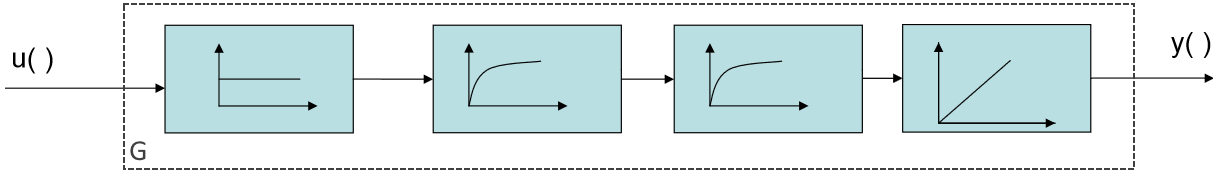
\includegraphics[width=16 cm]{foto/Transmitancja.png}
\caption{Wizualizacja dekompozycji obiektu o transmitancji G }
\label{fig:SCHEMAT}
\end{figure} 

\subsection{Dok�adna transmitancja dyskretna obiektu}
\begin{figure}[H]
\centering
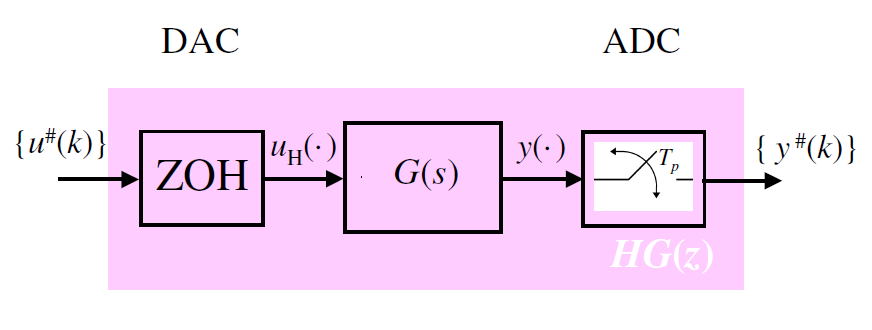
\includegraphics[width=16 cm]{foto/HGz.png}
\caption{Obiekt wraz z uk�adami DAC i ADC}
\label{fig:HGz}
\end{figure} 
Korzystaj�c z wzoru:
\begin{center}
\( HG(z)= \frac{z-1}{z}\mathcal{Z}(\mathcal{L}^{-1} (\frac{G(s)}{s}))= \frac{z-1}{z}\mathcal{D}(\frac{G(s)}{s})\) \\
\end{center}
dla czasu pr�bkowania \(T_p =0.04 \) otrzymano dok�adn� transmitancj� dyskretn� obiektu:
\begin{center}
\( HG(z)= \frac{6.344 \cdot 10^{-6} z^2 +  2.524 \cdot 10^{-5} z + 6.276 \cdot 10^{-6}}{z^3 - 2.979 z^2 + 2.958 z - 0.9788} \) \\
\end{center}

\subsection{Transmitancja widmowa}
Korzystaj�c z zale�no�ci:
\begin{center}
\( HG^*(j\omega )=HG(e^{T_pj\omega}) \)
\end{center}
obliczono transmitancj� widmow�:
\begin{center}
\( HG^*(j\omega )= \frac{6.344 \cdot 10^{-6} (e^{0.041j \omega})^2 +  2.524 \cdot 10^{-5} e^{0.041j \omega} + 6.276 \cdot 10^{-6}}{(e^{0.041j \omega})^3 - 2.979 (e^{0.041j \omega})^2 + 2.958 e^{0.041j \omega} - 0.9788} \)
\end{center}

\subsection{Transmitancja pseudocz�stotliwo�ciowa}
Transmitancja pseudocz�stotliwo�ciowa ma posta�:
\begin{center}
\( HG^{w*}(j\nu)= \frac{1.594 \cdot 10^{-6} j\nu^3 -  8.057 \cdot 10^{-4} j\nu^2 - 1.191 j\nu + 597.9}{j\nu^3 + 5.357 j\nu^2 + 3.986 j\nu}\) \\
\end{center}

Przybli�enie transmitancji pseudocz�stotliwo�ciowej:
\begin{center}
\( HG^{w*}_{est}(j\nu)= G(j\nu)(1-\frac{T_p}{2}j\nu)= \frac{- 0.3 j\nu + 150}{0.2509 j\nu + 1.344 j\nu+ s} \) \\
\end{center}

\begin{figure}[H]
\centering
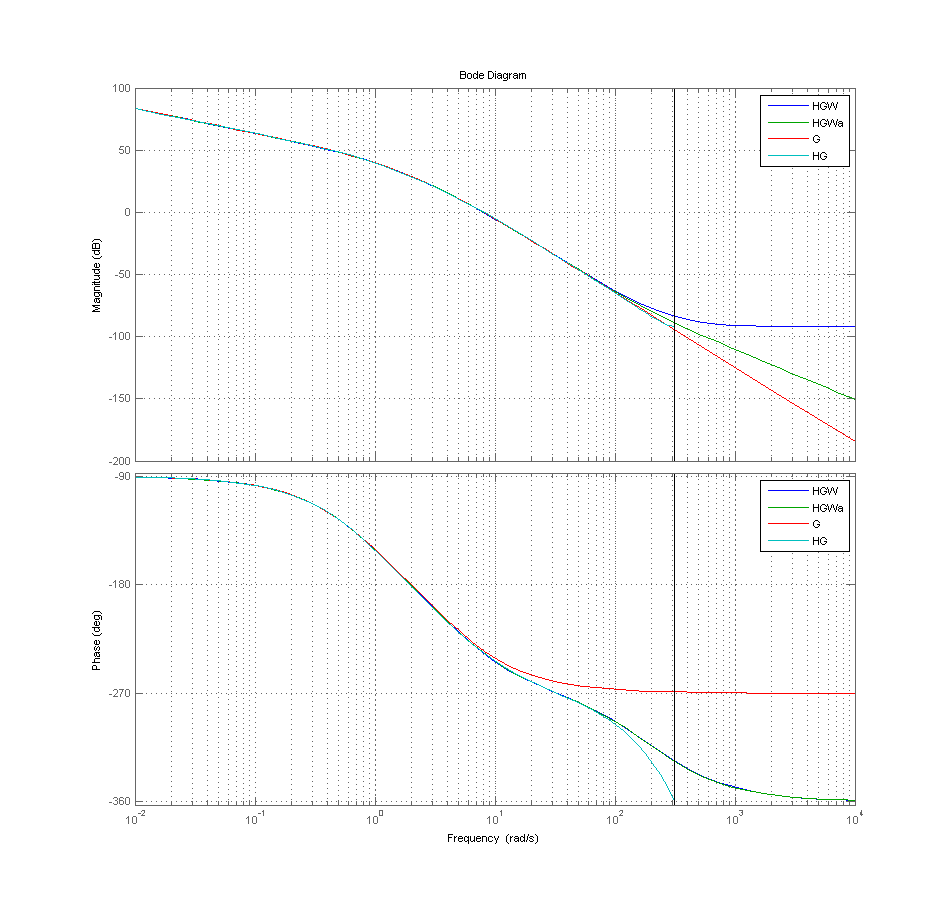
\includegraphics[width=16 cm]{photo/Transfer_functions.png}
\caption{Charakterystyka cz�stotliwo�ciowa transmitancji HGw*, HGw*est, HG* oraz G}
\label{fig:Bode}
\end{figure} 


\section{Projektowanie regulatora}
\subsection{Dob�r wzmocnienia regulatora}

Pierwszym krokiem zbli�aj�cym do obliczenia wzmocnienia by�o wyznaczenie obszaru zabronionego.
Korzystaj�c z definicji wymaga�: \\
\begin{center}
Maksymalna pr�dko��: \( r_1=1 \) \\
Maksymalne przyspieszenie: \( r_2=0.8 \) \\
Dok�adno��: \( \varepsilon=0.005 \) \\
\end{center}
obliczam wielko�ci \( \omega _a \) oraz \( L_gr \): \\
\begin{center}
\( \omega_a = \frac{r_2}{r_1}=0.8\) \\
\( L \ge \frac{1}{\epsilon} \frac{(r_1)^2}{r_2}\frac{1.16\cdot 4}{\pi}=369.2 \)
\end{center}
Na podstawie tych warto�ci wykre�lono wykres obszaru zabronionego. Naniesiono na niego r�wnie� wykres transmitancji \( HG^{w*}(j\nu) \). 
\begin{figure}[H]
\centering
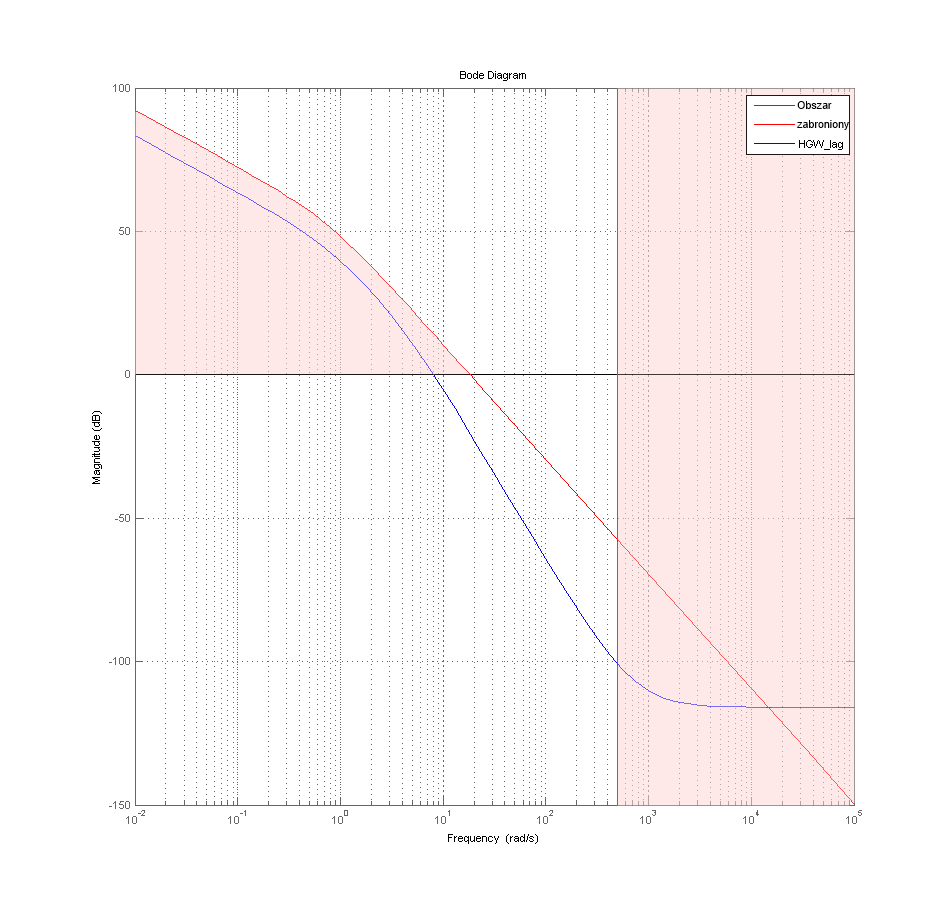
\includegraphics[width=16 cm]{photo/HGW_lag.png}
\caption{Obszar zabroniony}
\label{fig:HGW_lag}
\end{figure} 
Z analizy wykresu wynika, �e minimalne wzmocnienie, jakie powinien wprowadza� regulator wynosi  \( k_r=3 \)

\subsection{Dob�r nowej pulsacji granicznej}
Naturalna pseudopulsacja graniczna obiektu:  \( \nu _{gob}=8.0395 \). \\
Ograniczenie wynikaj�ce z wprowadzenia op�nienia: \( \nu _g < 110 \). \\
Przyj�to \( \nu _g = 80 \).\\
Z faktu przyj�cia, i� \( M_p = 1.4 \),
wynika, �e: \\ \( \nu _1 \le \nu _g \frac{M_p-1}{M_p}= 22.8571; \nu _2 \ge \nu _g \frac{M_p+1}{M_p}= 137.1429\) \\
Na podstawie przeprowadzonych symulacji dzia�ania regulatora, dobrano \( \nu _1=8,  \nu_2=400 \).

\begin{figure}[H]
\centering
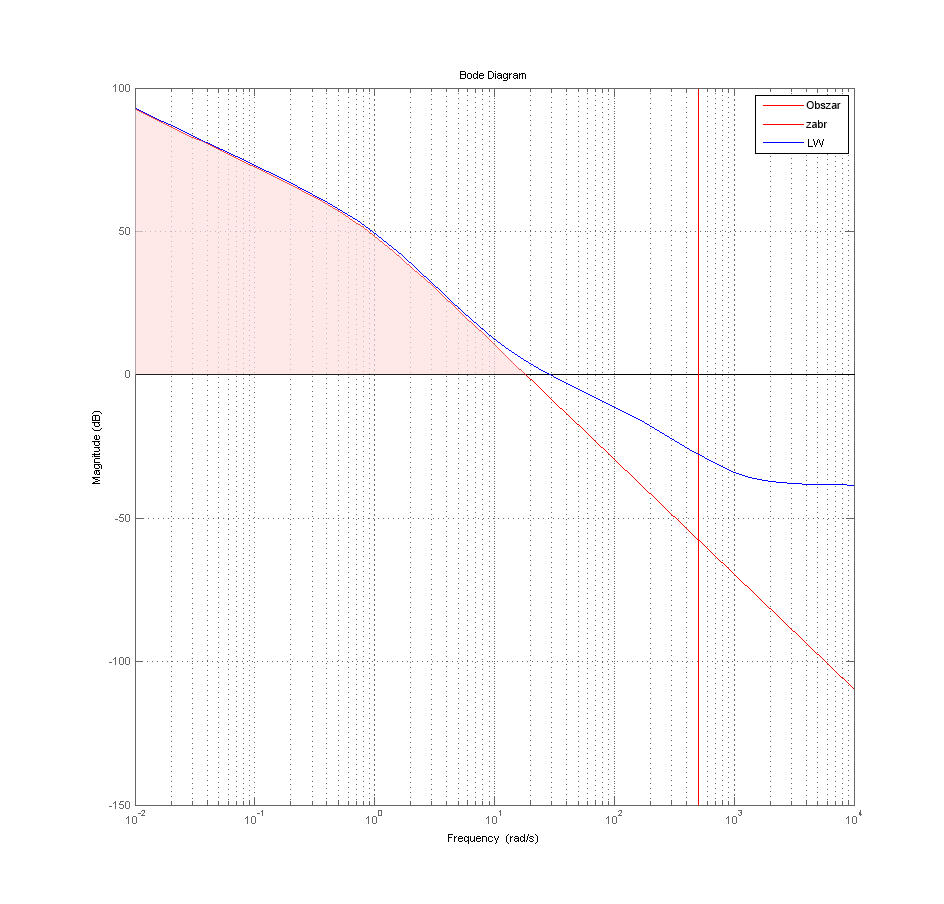
\includegraphics[width=16 cm]{photo/L_Bode.png}
\caption{Wykres Bodego dla obiektu z regulatorem}
\label{fig:HGW_lag}
\end{figure} 

\section{Regulator}
\subsection{Transmitancja}

Transmitancja regulatora wynosi:\\ 
\begin{center}
\( R(j \nu)=\frac{0.04664 j \nu^2 + 0.7482 j \nu + 3}{6.25e-06 j \nu^2 + 0.005 j \nu + 1} \)
\end{center}
Transmitancja impulsowa regulatora wynosi:\\ 
\begin{center}
\( R(z)=\frac{2378 z^2 - 4606 z + 2230}{z^3-0.2222 z^2 + 0.01235 z}\)
\end{center}
R�wnanie r�nicowe:\\
\begin{center}
\(u(k)=0.2222u(k-1)-0.01235u(k-2) + (2378e(k-1) - 4606e(k-2) + 2230)e(k-3)\)
\end{center}

\subsection{Stabilno��}

W celu zbadania stabilno�ci uk�adu wykonano wykres Nyquista oraz zbadano uk�ad poleceniem \textit{gain}.
\begin{figure}[H]
\centering
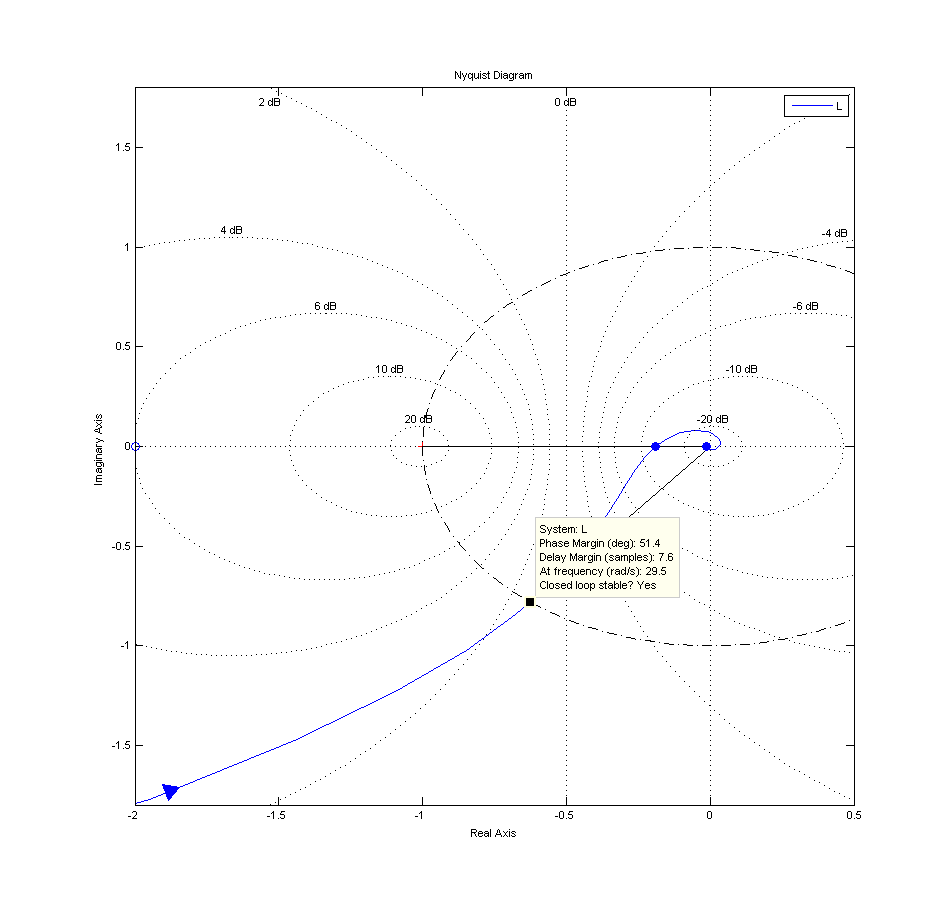
\includegraphics[width=16 cm]{photo/L_nyq.png}
\caption{Wykres Nyquista petli otwartej}
\label{fig:HGW_lag}
\end{figure} 
\begin{figure}[H]
\centering
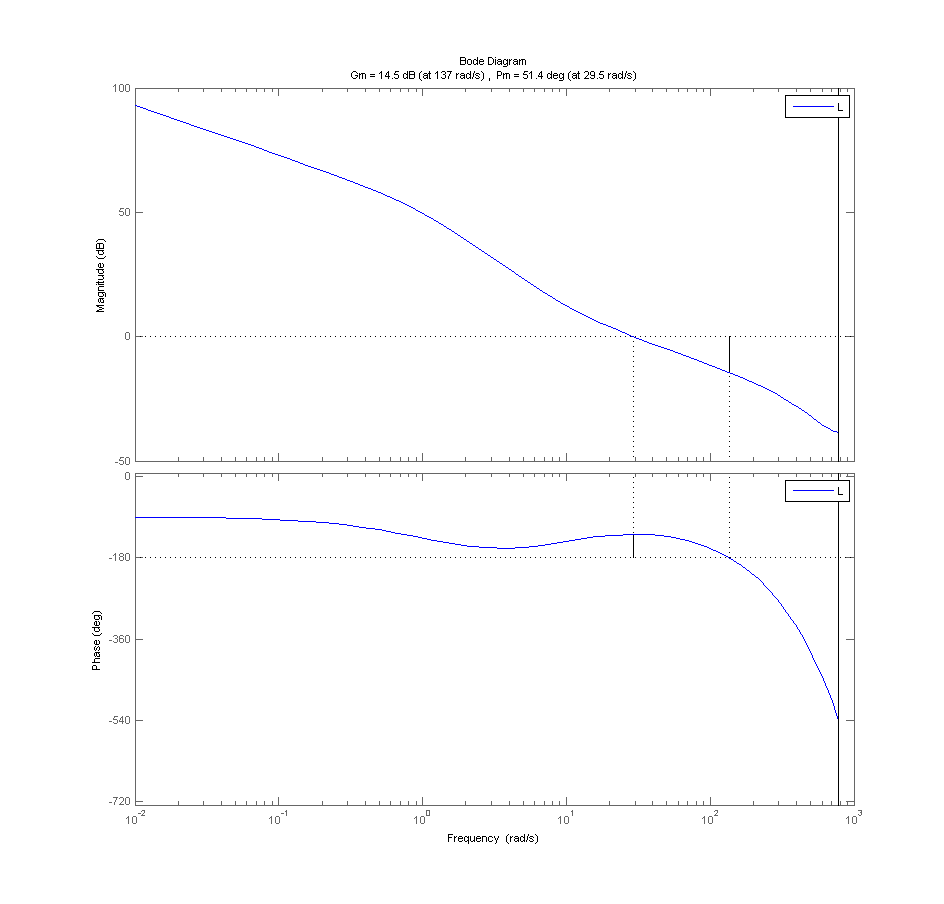
\includegraphics[width=16 cm]{photo/L_stab.png}
\caption{Wykres Bodego petli otwartej}
\label{fig:HGW_lag}
\end{figure} 

\subsection{Funkcje wra�liwo�ci}

W celu sprawdzenia reakcji uk�adu na spektrum cz�stotliwo�ci sygna�u wymuszenia
sporz�dzono wykresy:
\begin{itemize}
	\item funkcji wra�liwo�ci \( S=\frac{1}{1 + GR}\) oraz dope�niaj�cej funkcji wra�liwo�ci \( T=\frac{GR}{1 + GR}\)
	\item funkcji wra�liwo�ci na sterowanie \( Q=\frac{R}{1 + GR}\)
\end{itemize}

\begin{figure}[H]
\centering
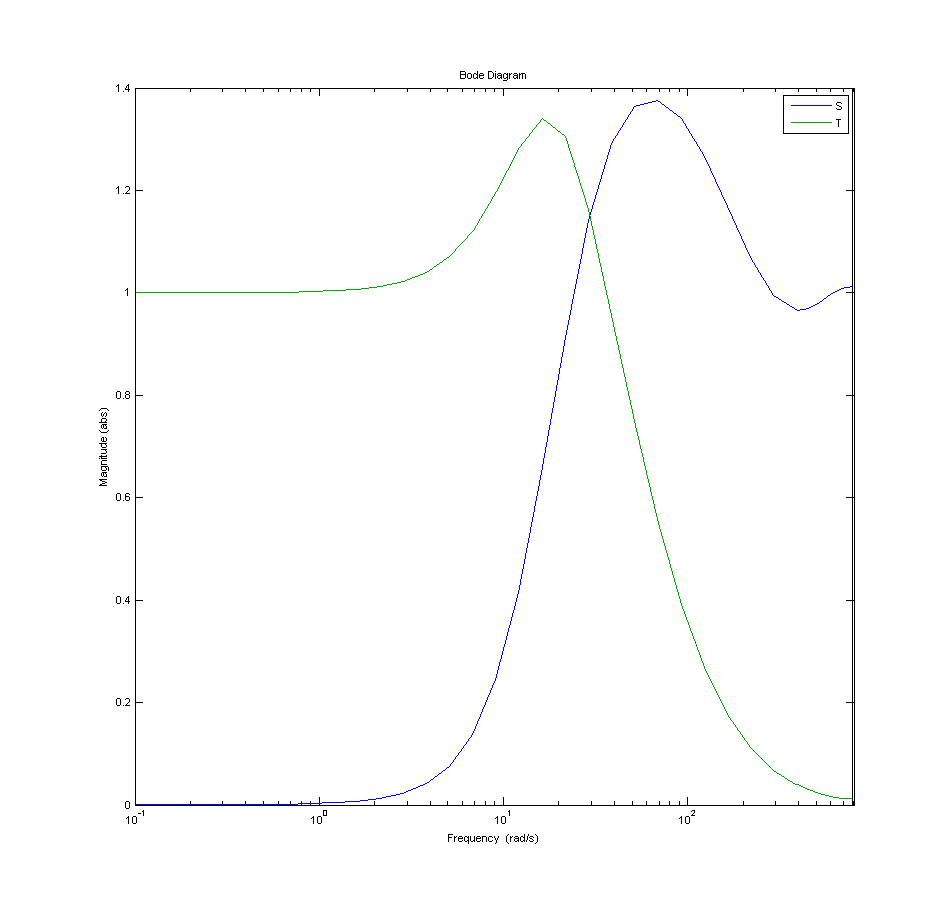
\includegraphics[width=16 cm]{photo/ST.png}
\caption{Wykres funkcji wra�liwo�ci oraz dope�niaj�cej funkcji wra�liwo�ci}
\label{fig:HGW_lag}
\end{figure} 
\begin{figure}[H]
\centering
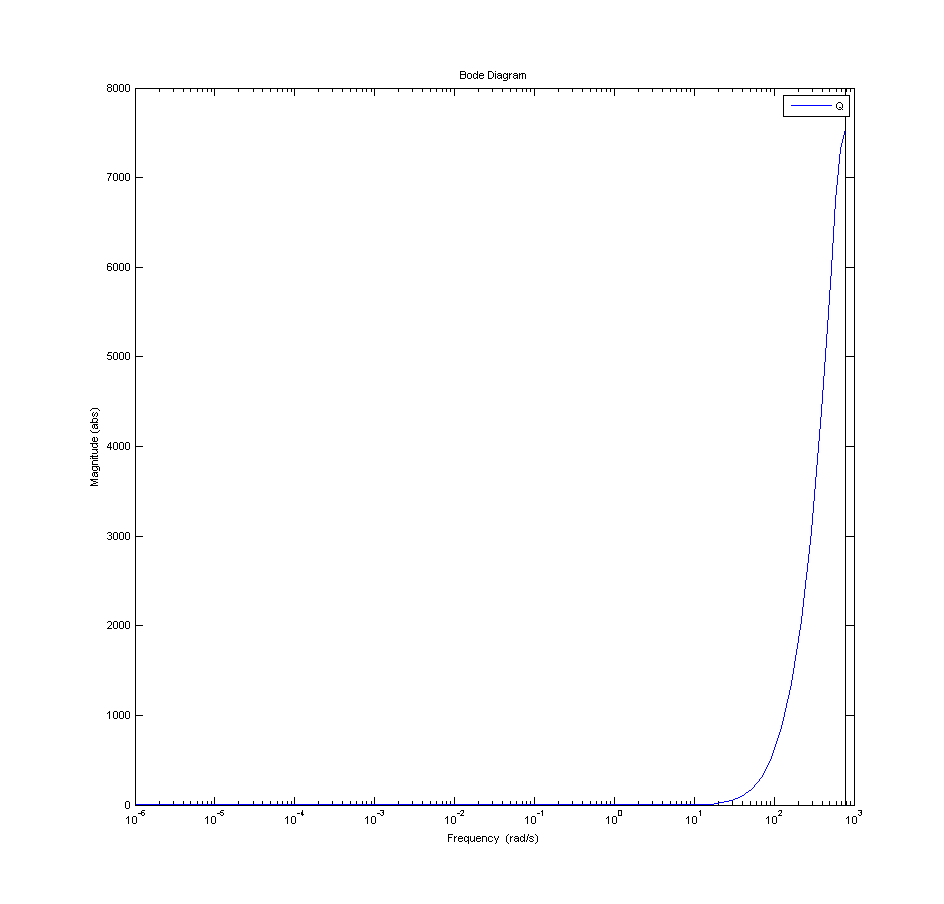
\includegraphics[width=16 cm]{photo/Q.png}
\caption{Wykres funkcji wra�liwo�ci na sterowanie}
\label{fig:HGW_lag}
\end{figure} 

\section{Odpowiedzi na zadane sygna�y}

\begin{figure}[H]
\centering
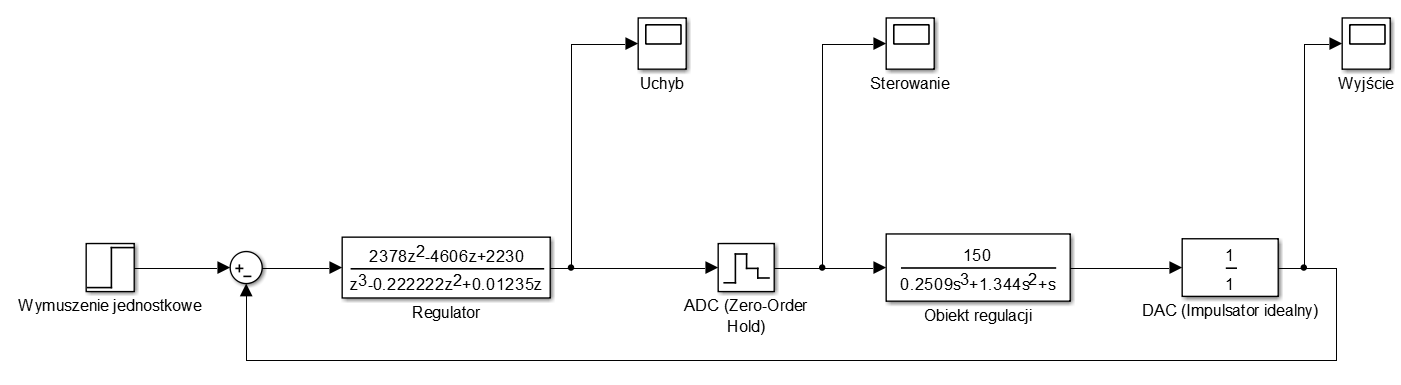
\includegraphics[width=16 cm]{photo/Simulink.png}
\caption{Schemat uk�adu}
\label{fig:HGW_lag}
\end{figure} 

\subsection{Odpowied� uk�adu na skok jednostkowy}
\begin{figure}[H]
\centering
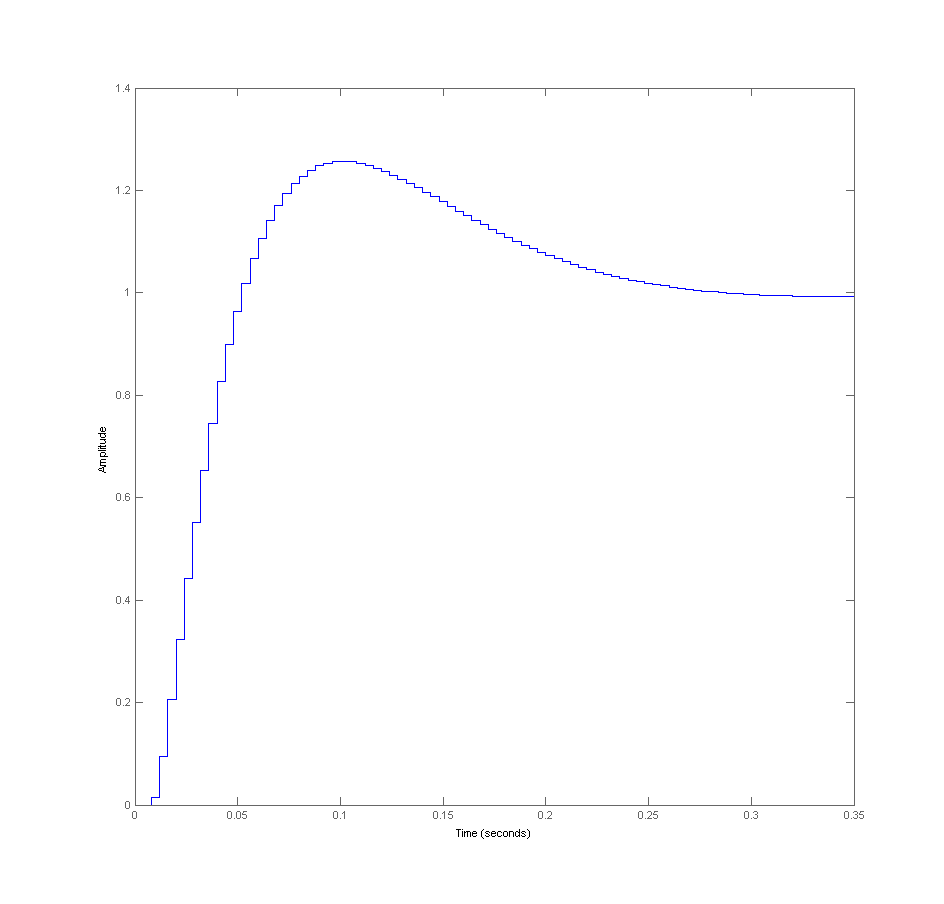
\includegraphics[width=16 cm]{photo/Step.png}
\caption{Odpowied� uk�adu na skok jednostkowy}
\label{fig:HGW_lag}
\end{figure} 

\subsection{Odpowied� uk�adu na skok o zadanej amplitudzie }
\begin{figure}[H]
\centering
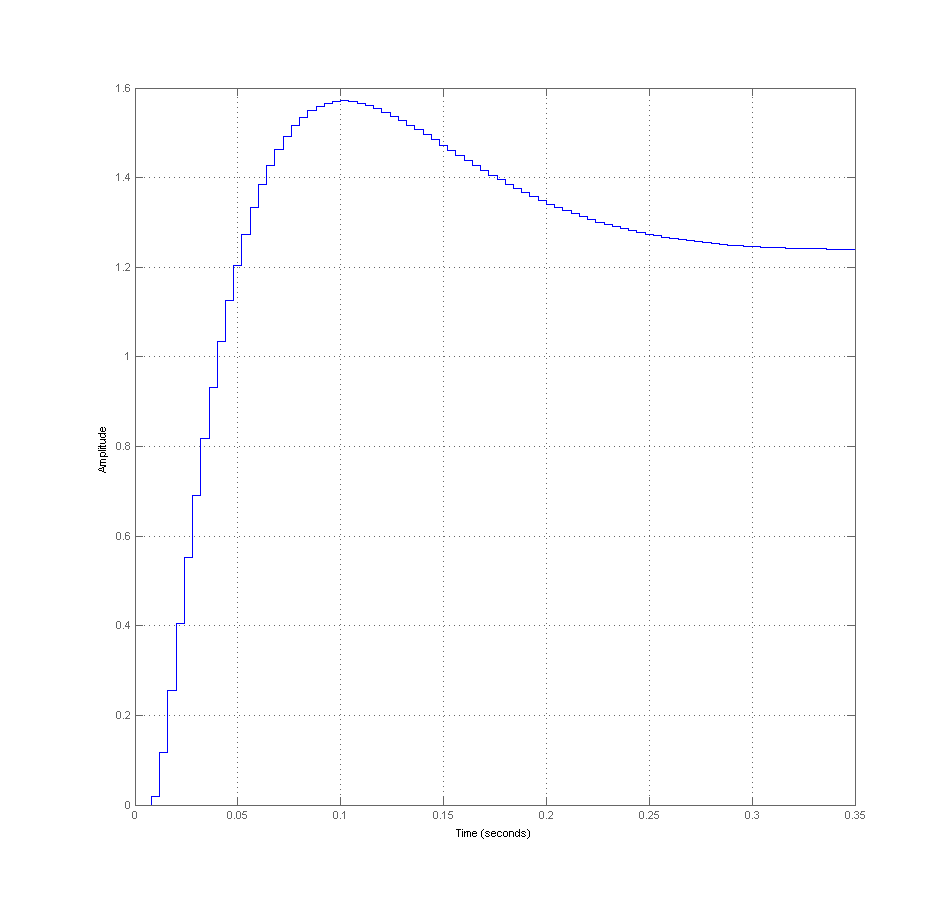
\includegraphics[width=16 cm]{photo/Step_R.png}
\caption{Odpowied� uk�adu na skok o zadanej amplitudzie}
\label{fig:HGW_lag}
\end{figure} 

\begin{figure}[H]
\centering
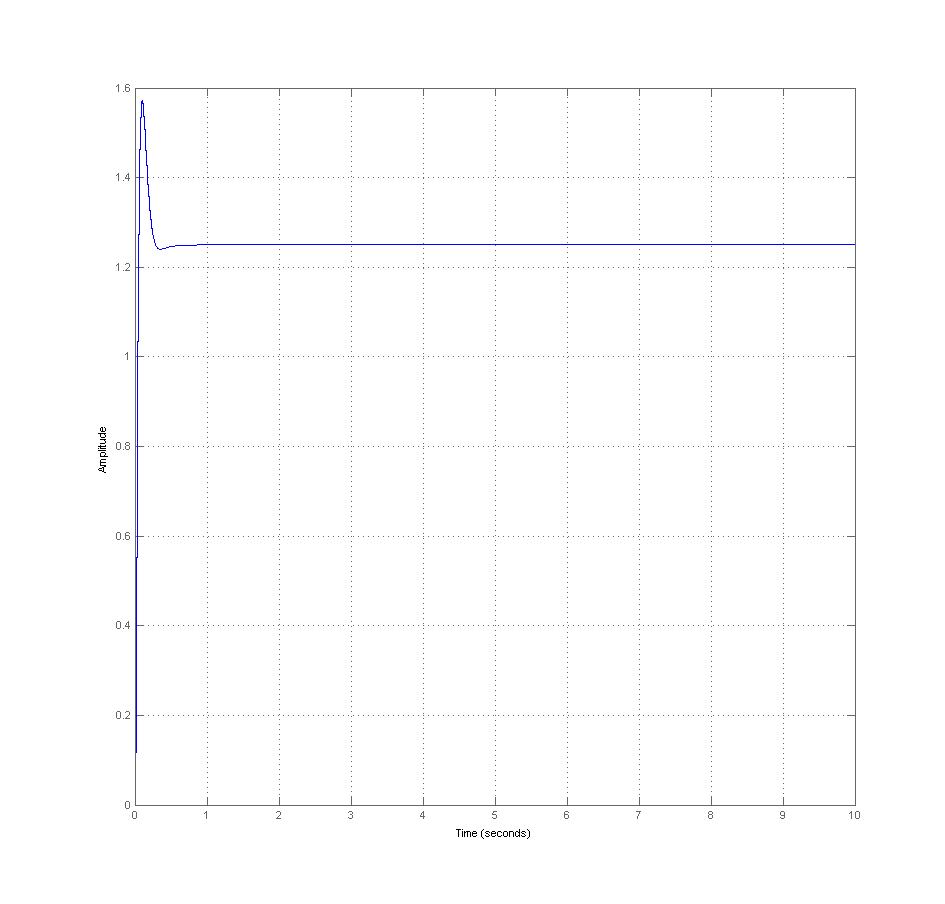
\includegraphics[width=16 cm]{photo/Step_R2.png}
\caption{Odpowied� uk�adu na skok o zadanej amplitudzie}
\label{fig:HGW_lag}
\end{figure} 

\subsection{Odpowied� uk�adu na wymuszenie sinusoidalne }
\begin{figure}[H]
\centering
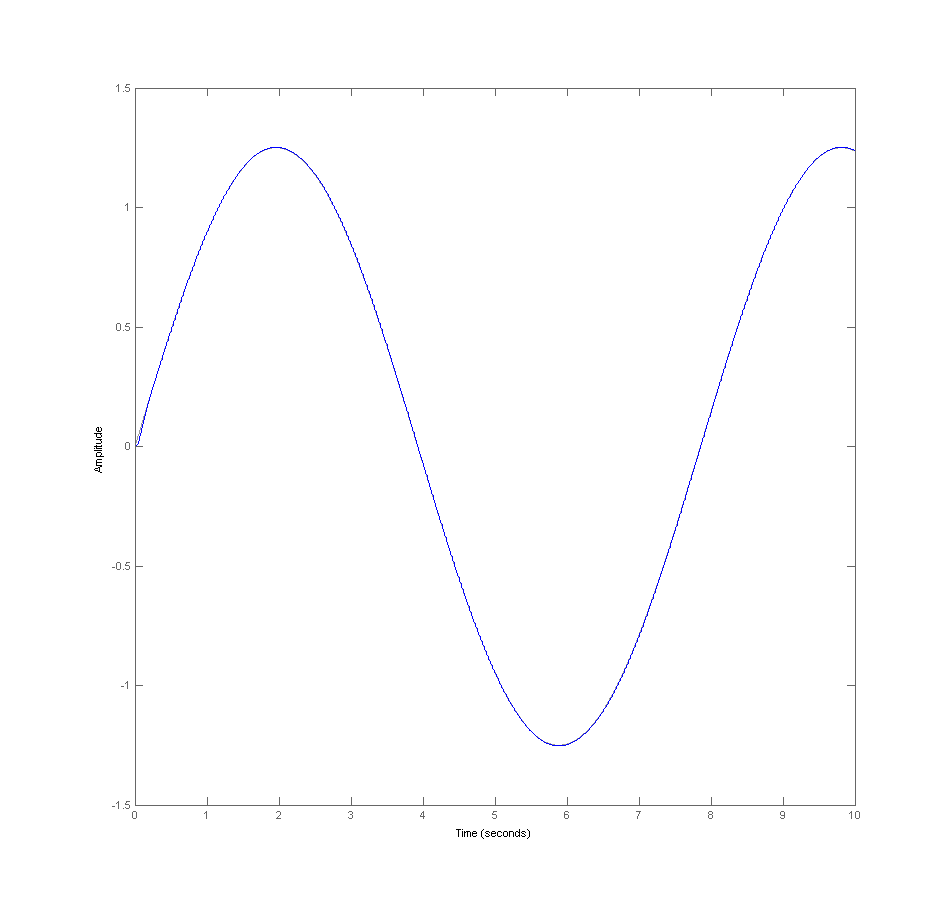
\includegraphics[width=16 cm]{photo/Sinus.png}
\caption{Odpowied� uk�adu na wymuszenie sinusoidalne}
\label{fig:HGW_lag}
\end{figure} 

\subsection{Odpowied� uk�adu na wymuszenie trapezowe }
\begin{figure}[H]
\centering
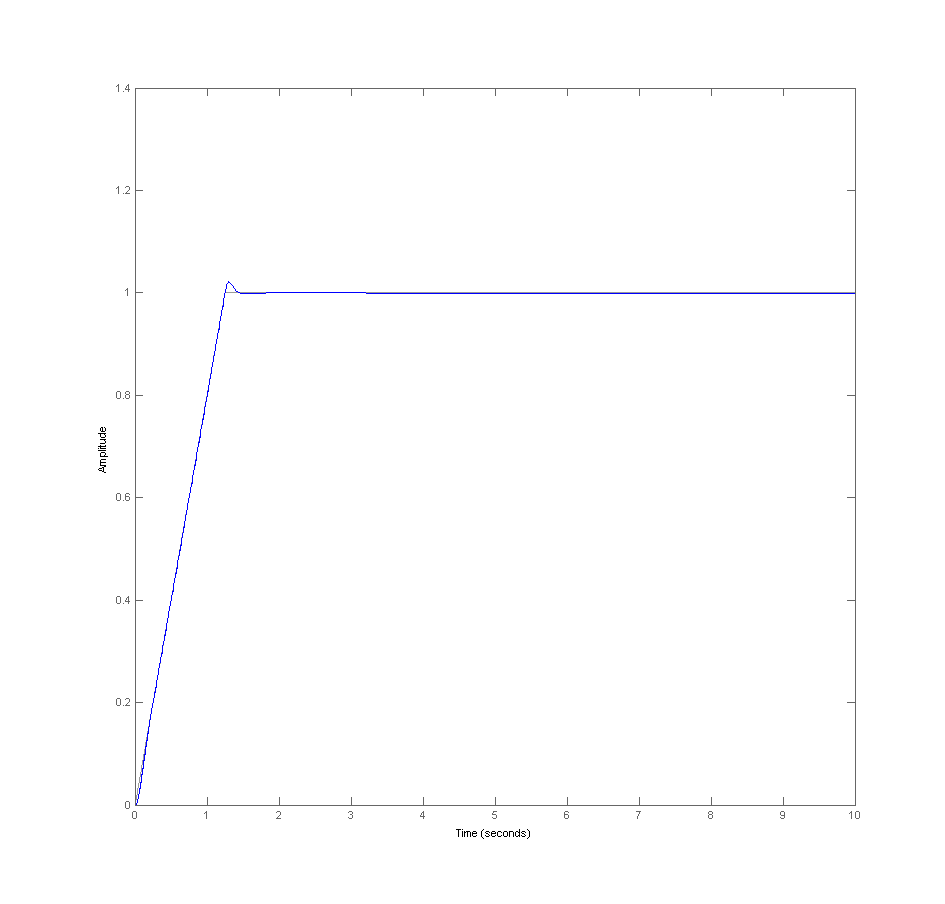
\includegraphics[width=16 cm]{photo/Trapezoidal.png}
\caption{Odpowied� uk�adu na wymuszenie trapezowe }
\label{fig:HGW_lag}
\end{figure} 

\begin{figure}[H]
\centering
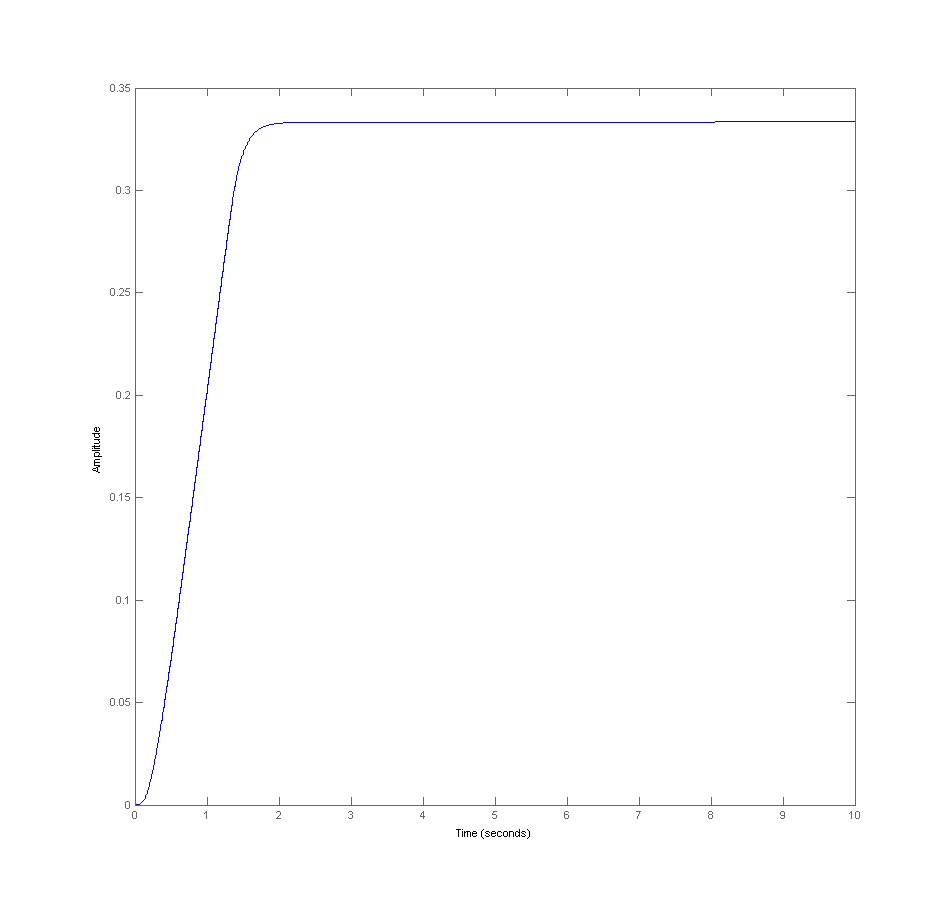
\includegraphics[width=16 cm]{photo/Control.png}
\caption{Sterowanie uk�adu przy wymuszeniu trapezowym }
\label{fig:HGW_lag}
\end{figure} 

\begin{figure}[H]
\centering
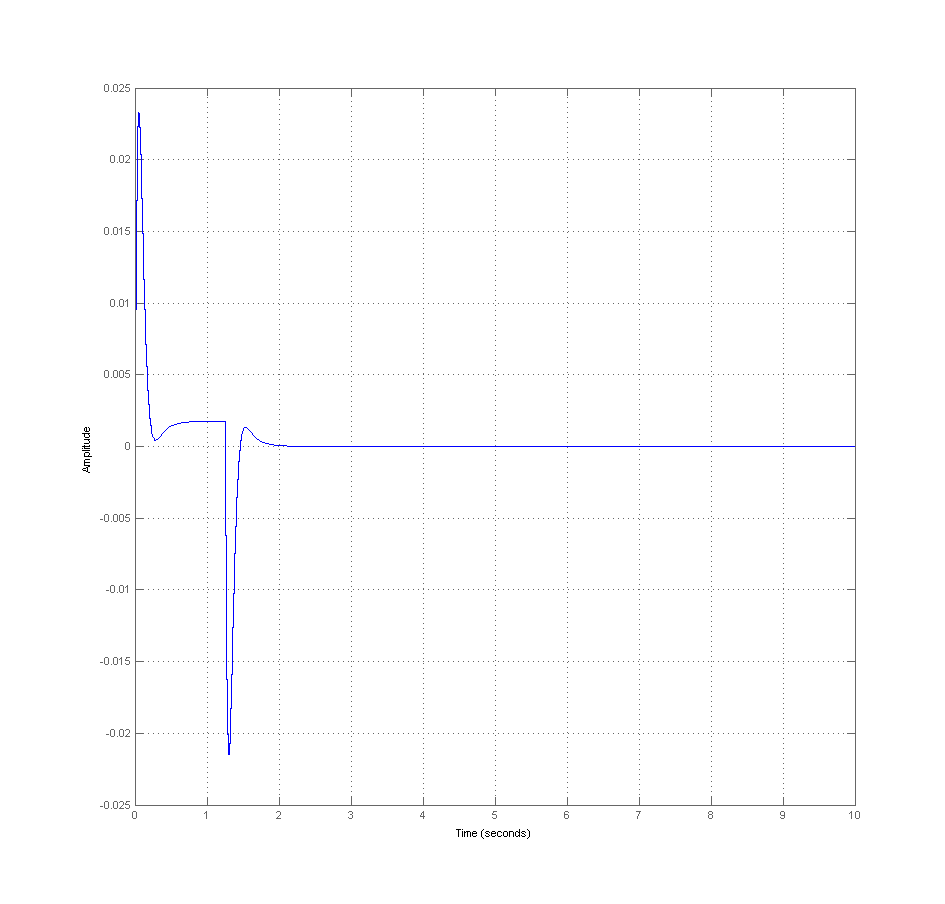
\includegraphics[width=16 cm]{photo/Error.png}
\caption{Uchyb uk�adu przy wymuszeniu trapezowym }
\label{fig:HGW_lag}
\end{figure} 
\chapter{Wnioski}

Celami projektu by�o wybra� czas pr�bkowania  \( T_p \) oraz dobra� tak transmitancj� regulatora dyskretnego \( R(z) \) , aby otrzyma� uk�ad regulacji spe�niaj�cy nast�puj�ce wymagania::

\begin{itemize}
\item uchyby po�o�eniowy i pr�dko�ciowy w stanie ustalonym s� najmniejsze z mo�liwych do osi�gni�cia,
\item  wymuszenia \( r \) o maksymalnej pr�dko�ci \( r_1 \)  i maksymalnym przyspieszeniu \( r_2 \) s� przenoszone
z uchybem nie wi�kszym ni� \( \varepsilon \) ,
\item  odpowied� uk�adu regulacji na skok jednostkowy charakteryzuje si� ma�� oscylacyjno�ci� i niezbyt
du�ym czasem ustalania, co jest zwi�zane z przyj�t� przez projektanta maksymaln� wielko�ci�
piku rezonansowego \( M_p \) uk�adu zamkni�tego,
\item  modu� sterowania \( u \) nie przekracza rozs�dnej granicy.
\end{itemize}

Niestety, pomimo wielokrotnych pr�b doboru zmiennych regulatora, nie uda�o si� doprowadzi� do sytuacji w kt�rej wszystkie z powy�szych wymaga� by�yby spe�nione. Pr�by wyeliminowania uchybu, b�d� przyspieszenia dzia�ania uk�adu skutkowa�y utrat� stabilno�ci (uk�ad schodzi� z zapasem modu�u poni�ej 6 dB). Aby unikn�� niestabilnie dzia�aj�cego uk�adu zdecydowano si� na pozostawienie regulatora w powy�szej formie, zdaj�c sobie spraw� z jego niedoci�gni��.

Projekt w znacz�cy spos�b przyczyni� si� do zrozumienia dzia�ania regulator�w oraz lepszego poznania oprogramowania in�ynierskiego: MatLAB (z pakietem Simulink), Rstudio oraz LaTeX.



\listoffigures

\begin{thebibliography}{1}
\bibitem{test1} Wo�niak A. {\em Materia�y do wyk�ad�w z Teorii Sterowania I}, Warszawa 2015
\bibitem{mataric}  de Larminat P., Thomas Y. {\em Automatyka Uk�ady Liniowe}, WNT, Warszawa, 1983
\end{thebibliography} 

\end{document}
